\documentclass[11pt]{article}

% basic packages
\usepackage[margin=2cm]{geometry}
\usepackage[pdftex]{graphicx}
\usepackage{amsmath,amssymb,amsthm}
\usepackage{custom}

% page formatting
\usepackage{fancyhdr}
\pagestyle{fancy}

\renewcommand{\sectionmark}[1]{\markright{\textsf{\arabic{section}. #1}}}
\renewcommand{\subsectionmark}[1]{}
\lhead{\textbf{\thepage} \ \ \nouppercase{\rightmark}}
\chead{}
\rhead{}
\lfoot{}
\cfoot{}
\rfoot{}
\setlength{\headheight}{14pt}

\linespread{1.03} % give a little extra room
\setlength{\parindent}{0.2in} % reduce paragraph indent a bit
\setcounter{secnumdepth}{2} % no numbered subsubsections
\setcounter{tocdepth}{2} % no subsubsections in ToC

\begin{document}

% make title page
\thispagestyle{empty}
\bigskip \
\vspace{0.1cm}

\begin{center}
{\fontsize{36}{36} \selectfont \bf \sffamily Electromagnetism Notes}
\vskip 24pt
{\fontsize{18}{18} \selectfont \rmfamily Conor Redington} 
\vskip 24pt
\end{center}

% make table of contents
\newpage
\microtoc
\newpage

% main content
\hypertarget{electromagnetism}{%
\section{Electromagnetism}\label{electromagnetism}}

\emph{trying to aggregate}

\hypertarget{broad-strokes}{%
\section{Broad strokes}\label{broad-strokes}}

\begin{itemize}
\tightlist
\item
  We've two types of fields, electric and magnetic.
\item
  There's two types of energies to these fields, electric potential and
  magnetic potential (?).
\item
  Induction. Faraday's law combines these two fields experimentally in
  that a moving loop in a magnetic field generates an emf in that loop
  (hence, an electric field).
\item
  Why does this happen?
\item
  Maxwell then said, if a changing magnetic field can induce an electric
  field, could a changing electric field induce a magnetic field.
\end{itemize}

\hypertarget{electrostatics}{%
\section{Electrostatics}\label{electrostatics}}

\emph{following along from Chpt 21 in University Physics}

\hypertarget{electric-charge}{%
\subsection{Electric Charge}\label{electric-charge}}

\begin{itemize}
\tightlist
\item
  Charge is a property of particles, like mass. It's what determines
  their interaction with the \emph{electromagnetic force}
\item
  The unit of charge is the coulomb. Because conglomerations of
  particles are more common in nature a coulomb is the negative charge
  of \(6\times10^{18}\) electrons
\item
  When we're trying to determine the affect a charged particle has on
  the space around it, we define a field. That is, when you place
  another charged particle (the set of things affected by the field) in
  the space around it, what force will it experience? We define the
  field as the force per unit of charge placed in it. So you then have
  some determinism as to what force will be experienced by a charge you
  place into the field (provided you're using the same units as the test
  charge)
\end{itemize}

\hypertarget{electric-current-and-electromotive-force}{%
\section{Electric Current and Electromotive
Force}\label{electric-current-and-electromotive-force}}

\emph{following along from chapter 25 of University Physics}

\begin{itemize}
\item
  Current is any \emph{net} motion of charge from one region to another.
\item
  Free electrons are naturally occurring in a conducting material.
\item
  If an electric field is applied the electrons move with a force
  dictated by that field. They `bump' into positive ions and in general
  there is a mass of electrons slowly crawling their way along the
  conductor. They do this at a velocity called the \emph{drift
  velocity}.
\item
  The kinetic energy of the electrons is transferred to the ions when
  they collide, this causes a rise in temperature of the material.
  \textbf{Most of the work done by the field goes into heating up the
  material.}
\item
  Do electrons collide with one another? Presumably yes, but they're
  much smaller than the atoms so maybe it's less frequent.
\item
  In conductors the movement after the application of a field is done by
  electrons. In \emph{conventional current} the free charges are assumed
  to be positive. Current is a scalar so direction doesn't matter. It's
  the net charge flowing through a cross sectional area per unit time
\item
  When a electric field is applied all free moving electrons go one
  direction and all free moving positive charges go the other.
\item
  Drift velocity is in the same direction as the field if we assume that
  the free moving charges are positive.
\item
  For metals at a given temperature, the current density (\(\vec{J}\))
  is generally proportional to the resistivity of the material. Current
  density is current for a given cross sectional area.
\item
  \[\rho = \frac{E}{J}\]
\item
  Current is the rate of change of charge, it can also be useful to look
  at current per unit area, the rate of change of charge through a
  particular area.
\item
  \[i = \frac{dQ}{dt}\]
\item
  \[dQ = qnAv_ddt; Av_ddt \text{ basically a small volume of charge}\]
\item
  \[\vec{J} = \frac{i}{A} = nq\vec{v_d}\]
\item
  \begin{quote}
  For simple materials such as metallic conductors, the current density
  is proportional to the electric field.
  \end{quote}
\item
  The proportionality constant is known as conductivity.
\end{itemize}

\hypertarget{ohms-law}{%
\subsubsection{Ohms Law}\label{ohms-law}}

\emph{Chapter 26 Halliday} * The essence of Ohm's law is that a plot of
i versus V is linear for a conductor. When the resistivity is
independent of magnitude and direction of the field. * All homogenous
materials obey Ohm's law within some range of values of electric field.

\hypertarget{power}{%
\subsection{Power}\label{power}}

\begin{itemize}
\tightlist
\item
  When a potential difference exists in a circuit, the potential drop
  that an electron experiences must be transferred into some other form
  of energy (by the conservation law).
\item
  The rate of this transfer \(dU/dt\) is
\item
  \[P = iV\]
\item
  This applies to the transfer of energy of all kinds.
\item
  \(P = i^2R\) and \(P = \frac{v^2}{R}\) applies to resistive
  dissipation (energy loss due to collisions with atoms in the
  resistor).
\end{itemize}

\hypertarget{electric-field-lines}{%
\section{Electric field lines}\label{electric-field-lines}}

\begin{itemize}
\tightlist
\item
  Indicate the direction of the electric field.
\item
  Magnitude of the electric field is proportional to the number of lines
  crossing a unit area. The closer the lines, the stronger the field.
\item
  Start on positive charges and end on negative charges. The number of
  starting lines is proportional to the charge.
\end{itemize}

\hypertarget{electric-flux}{%
\subsection{Electric flux}\label{electric-flux}}

\begin{itemize}
\tightlist
\item
  \emph{Gauss' law} relates electric field at points on a closed
  Gaussian surface (just an imaginary concentric sphere surrounding a
  charge) to the net charge of the enclosed surface
\item
  If we know the charge, we can determine the field at a point, if we
  know a field we can determine the source charge. We need a measure of
  the field at a point on this Gauss surface.
\item
  For a tiny patch of a flat surface \(\Delta{A}\) the amount of
  electric field going through this patch is \(Ecos(\theta)\Delta{A}\)
  because if the field is perpendicular to the surface the x component
  is the only portion of it acting on the surface. The `amount' of
  electric field `piercing' this area is \(\Delta{\phi}\)
\item
  \(\Delta{\phi} = E\cdot\Delta{A}\) dot product will get the x
  component of the electric field
\item
  The total flux can then be \(\phi = \int{\vec{E} \cdot d\vec{a}}\)
  vector integrals?
\item
  The flux allows us to know directionality too. Because A is a vector
  also, meaning that if E switches direction the angle \(\theta\)
  becomes 180 and the dot product flips.
\item
  An inward piercing field is negative flux and an outward piercing
  field is positive flux
\item
  The SI unit of flux is \(N/m^2/C\) it's a magnitude, an amount.
\item
  \(\oint{\vec{E} \cdot d\vec{A}}\)
\item
  The area vector A is always perpendicular to the surface and always
  points away from the interior of the Gaussian surface
\item
  Gauss' law: \(\epsilon_0 \oint{\vec{E} \cdot d\vec{A}} = q_{enc}\)
\item
  If there is a Gaussian surface with no charge enclosed, any field
  lines entering it also leave it.
\end{itemize}

\hypertarget{energy-of-electric-field}{%
\section{Energy of electric field}\label{energy-of-electric-field}}

\begin{itemize}
\tightlist
\item
  \textbf{Electric potential} (or potential) is the electric potential
  energy per unit charge.
\item
  Potential at some point is dependent on what is chosen to have zero
  potential as potential is only useful as a quantity of change.
\item
  Often, the ground is chosen. If something is 50 volts the difference
  in potential between it and the ground is 50V.
\item
  In some case (I'm think specifically in bonding models here) the
  potential is chosen to be zero at an infinite distance
  (\(r \rightarrow \infty\)).
\item
  Potential difference is a measure of how much energy a charge can
  acquire, or, how much work it can do.
\item
  Important to relate the notion of charge \textbf{and} voltage defining
  the energy transferred in some movement.
\item
  The work done by a charge in moving from a to b is the negative of the
  change in potential energy.
\item
  \[W = -q(V_b - V_a) = -qV_{ba}\]
\item
  W is force by distance. \(W = qEd\) where d is the distance from a to
  b
\item
  \[-qV_{ab} = qEd \rightarrow E = -\frac{V_{ab}}{d}\]
\item
  What is the electric potential for a point charge?
\item
  The main ease of use it seems is that potentials add as scalars
  whereas fields add as vectors.
\end{itemize}

\hypertarget{magnetism}{%
\section{Magnetism}\label{magnetism}}

\begin{itemize}
\tightlist
\item
  Elementary particles have an intrinsic magnetic field around them.
\item
  Magnetic poles always appear in pairs, their has not been found to
  exists an isolated south or north pole of a magnet
\item
  The nature of the magnetic force is different to the electric force.
  Through experimentation with velocities of particles it's found that
  if we want to know a magnetic field \(B\) we measure the force
  experienced by charges fired through it at different velocities. There
  is a line where the particle experiences no force and all forces
  experienced after that seem proportional to \(vsin(\theta)\) where
  \(\theta\) is the angle between velocity vector and zero force line.
  The force of the field always seems to act perpendicular to the
  velocity vector.
\item
  \[\vec{F_b} = q\vec{v} \times \vec{B}\]
\item
  The force of the magnetic field relies on the movement of charge
\item
  \(\vec{F_b}\) can never change the particle speed because it's always
  acting perpendicular, so it doesn't contribute to it's kinetic energy.
  It can change it's direction though which is changing its
  acceleration?
\item
  The magnetic force on a conductor when you've a moving charge through
  it is \(\vec{F_b} = I\vec{l} \times \vec{B}\) If you let l become
  infinitely small then you can find the force at all points along any
  shaped conductor
\end{itemize}

\hypertarget{electromotive-force}{%
\section{Electromotive Force}\label{electromotive-force}}

\begin{itemize}
\tightlist
\item
  the influence that makes current flow from lower to higher potential
  is electromotive force. It's an energy per unit charge though, not a
  force.
\item
  If you make a circuit with an electric field pointing one direction.
  At some point along the field work has do be done for the free
  particles to reset at the top of the circle. In the sense that they
  need to overcome the negative work being done on them by the field
  when they get over halfway around the circle. The work done by the emf
  then is just the opposite of the work done by the field.
\item
  You would want another electric field at the bottom of the circle to
  give the free particles a `push' against the oncoming field
\item
  There is internal resistance in the emf source too so the actual
  current flow in the circuit must take this into account too.
\item
  SI unit: Joule/coulomb as it's a measure of the work that needs to be
  done per unit charge to lift it up the energy well.
\end{itemize}

\hypertarget{induction}{%
\section{Induction}\label{induction}}

\begin{itemize}
\tightlist
\item
  Transfer of mechanical energy to electrical energy.
\item
  If you move a magnet towards a wire it can induce a current
  proportional to the speed of it's motion and the pole directed towards
  the loop current. The current is `induced' and the work done per unit
  charge to induce that current is the induced emf.
\item
  A current and emf is induced when the number of magnetic field lines
  passing through a loop is changing.
\item
  The emf here, is the energy provided to induce the motion of the
  current that we see. A force that causes free particles to move away
  from lowest potential.
\item
  If we define magnetic flux (field perpendicular to a surface) as
  \(\phi_B = \oint{\vec{B}d\vec{A}}\) where area is the surface area of
  the loop. Faraday's law can then be: the magnitude of the emf induced
  is the time rate of change of the magnetic flux
  \(emf = -\frac{d\phi_B}{dt}\) (Faraday's law)
\item
  If the same flux passes through N loops \(emf = -N\frac{d\phi_B}{dt}\)
\end{itemize}

\hypertarget{lenzs-law}{%
\section{Lenz's law}\label{lenzs-law}}

\begin{itemize}
\tightlist
\item
  An induced current will produce a magnetic field that will oppose the
  magnetic flux that induced the current.
\item
  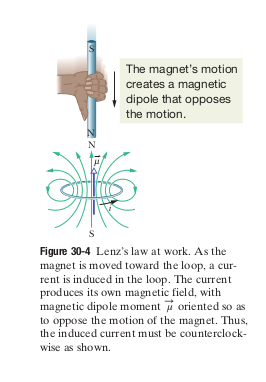
\includegraphics{physics/img/lenzlaw.png}
\end{itemize}

\hypertarget{capacitance}{%
\section{Capacitance}\label{capacitance}}

\begin{itemize}
\tightlist
\item
  The capability of a material to store electric charge.
\end{itemize}

\hypertarget{explain-how-a-battery-works}{%
\subsection{Explain how a battery
works}\label{explain-how-a-battery-works}}

\href{https://www.youtube.com/watch?v=4-1psMHSpKs}{Cool vid and
visualisation}

\hypertarget{circuits}{%
\section{Circuits}\label{circuits}}

\emph{Chapters 26 + 27}

Just like mechanical energy we need a way of periodically delivering
energy (engine). This is done for electrical energy through circuits.

In a circuit, voltage acts as a pump. Resistors or the load act as
something that will extract the energy and hopefully do useful work with
it (or just dissipate it as heat).

\textbf{Loop rule}: The algebraic sum of the changes in potential
encountered in a complete traversal of any loop of a circuit must be
zero.

\textbf{Junction rule}: The sum of the currents entering any junction
must be equal to the sum of the currents leaving that junction.

The circuit diagram is kind of like a map of potential, just like a
point in space under gravity.

\hypertarget{capacitors}{%
\subsection{Capacitors}\label{capacitors}}

\emph{from chapter 25 of Halliday}

\begin{itemize}
\tightlist
\item
  A device in which electrical energy can be stored.
\item
  The \emph{capacitance} is a measure of how much charge is required to
  achieve a potential difference V between two plates.
\item
  \[q = CV\]
\item
  Capacitors in parallel.
\item
  \[C_{eq} = \sum^n{j = 1}C_j\]
\item
  Capacitors in series.
\item
  \[C_{eq} = \sum^n{j = 1}\frac{1}{C_j}\]
\end{itemize}

\hypertarget{charging-a-capacitor-rc-circuit}{%
\subsubsection{Charging a Capacitor (RC
circuit)}\label{charging-a-capacitor-rc-circuit}}

\emph{chapter 27}

\begin{itemize}
\tightlist
\item
  In a simple series RC circuit, if we want to know the charge on a
  capacitor at time t.
\item
  \(V = iR - \frac{q}{C} = 0\)
\item
  \(\frac{q}{C}\) is the pd across the capacitor.
\item
  \(R\frac{dq}{dt} + \frac{q}{C} = V\)
\item
  We need to solve this for all q through time.
\item
  The solution is \(q(t) = CV(1 - e^{-t/RC})\)
\item
  The derivative of \(q(t)\) is \(i = \frac{V}{R}e^{-t/RC}\)
\item
  The voltage across the capacitor varies as
  \(V_C = V(1 - (1 - e^{-t/RC})\)
\end{itemize}

\hypertarget{lc-oscillations}{%
\subsubsection{LC Oscillations}\label{lc-oscillations}}

\begin{itemize}
\tightlist
\item
  At any time t, the energy store in a capacitor is
  \(U_E = \frac{q^2}{2C}\).
\item
  At any time t, the energy stored in the magnetic field of an inductor
  is \(U_B = \frac{Li^2}{2}\).
\item
  If we assume a circuit with and inductor and a capacitor where the
  capacitor is \emph{fully charged} to begin with.
\item
  There is an oscillating transfer of charge between the two components
  at a frequency \(f\) and angular frequency \(\omega = 2\pif\).
\item
  This would continue indefinitely if not for resistance (energy loss in
  the wires).
\end{itemize}

\hypertarget{differential-equation-for-lc}{%
\paragraph{Differential Equation for
LC}\label{differential-equation-for-lc}}

\begin{itemize}
\tightlist
\item
  An analogy is made to a block and spring system.
\item
  \[U = U_b + U_E = U_E = U_B = \frac{Li^2}{2} + \frac{q^2}{2C}\].
\item
  \[\frac{dU}{dt} = L\frac{d^2q}{dt^2} + \frac{1}{C}q = 0\].
\item
  The solution to this equation is \(q = Qcos(\omegat + \phi)\) and
  \(i = Isin(\omegat + \phi)\) where \(I = \omegaQ\).
\item
  This is a solution provided \(\omega = \frac{1}{\sqrt{LC}}\).
\item
  This is considered a \emph{free oscillation}.
\end{itemize}

\hypertarget{alternating-current}{%
\section{Alternating Current}\label{alternating-current}}

\begin{itemize}
\tightlist
\item
  In an RLC circuit, the rate a which natural oscillations occur might
  be at some frequency \(\omega\).
\item
  Introducing an emf that is oscillating introduces a driving force, a
  forced oscillation.
\item
  We assume that there may be a lag, due to reactance in the circuit
  between the emf and it's current, this is represented with
  \(\omega_dt - \phi\).
\end{itemize}

\hypertarget{driven-oscillation}{%
\subsection{Driven Oscillation}\label{driven-oscillation}}

\begin{itemize}
\tightlist
\item
  An oscillating emf drives current and a potential difference through
  the circuit by \(v(t) = Vsin(\omega_dt)\).
\item
  The resistance of the circuit at a time t is
  \(v_r(t) = V_rsin(\omega_dt)\).
\item
  When resistance amplitude varies with voltage current, then, has no
  phase shift.
\item
  \(i_R = I_Rsin(\omega_dt)\).
\end{itemize}

\hypertarget{phasors}{%
\paragraph{Phasors}\label{phasors}}

\begin{itemize}
\tightlist
\item
  The angle is makes with the horizontal is \(\omegat\).
\item
  The angle between vectors in this space is the phase difference
  between them.
\item
  The value at a time t is the projection on to the real axis
  (horizontal in most cases).
\item
  When sine is used below, it's not the phasor representation. The
  phasors representation allows us to put the oscillation of interest on
  the x axis (real axis) for manipulation. Cos is just sin `shifted' by
  90 degrees.
\end{itemize}

\hypertarget{capacitive-reactance}{%
\subsection{Capacitive Reactance}\label{capacitive-reactance}}

\begin{itemize}
\tightlist
\item
  If the capacitor voltage is the same as the driving voltage we have
  \(v_c = V_Csin\omega_dt\).
\item
  To derive the current, we look at the charge on the capacitor at this
  time t, \(q_c = Cv_c = CV_Csin\omega_dt\).
\item
  Current is then \(dq_C/dt = \omega_dCV_Ccos\omega_dt\).
\item
  Capacitive reactance is \(X_C = \frac{1}{\omega_dC}\). It's unit is
  the ohm (look at time constant).
\item
  \[i_C = (\frac{V_C}{X_C})sin(\omega_dt + 90)\].
\item
  From \protect\hyperlink{Alternatingux5cux2520Current}{above}
  \(i_c = I_Csin(\omega_dt - \phi)\) so the phase is shifted back by 90
  degrees for a capacitive load.
\item
  The voltage and current amplitude are linked by \(V_C = I_CX_C\).
\end{itemize}

\hypertarget{inductive-reactance}{%
\subsection{Inductive Reactance}\label{inductive-reactance}}

\begin{itemize}
\tightlist
\item
  The same steps work for an inductive load.
\item
  Inductive reactance is \(X_L = \omega_dL\). It's unit is the ohm (look
  at time constant).
\item
  The voltage and current amplitude are linked by \(V_L = I_LX_L\).
\item
  Here, the phase is plus 90 degrees, which means the current through
  the inductor lags the voltage through the inductor. Because the
  convention says that current will by some negative phase of voltage,
  when you sub in a positive value and put it on a phasor diagram, the
  current phasors rotates clockwise a phase \(\phi\) from the voltage.
\end{itemize}

\hypertarget{power-1}{%
\subsection{Power}\label{power-1}}

In the RLC circuit, the source of energy is the alternating current.
Some of this energy is stored in the magnetic field of the inductor, the
electric field of the capacitor or dissipated as heat from the resistor.

\begin{itemize}
\tightlist
\item
  If we take the average power \(P = I_msin^2(\omegat)R\) the average
  value of \(sin^2\) is 1/2.
\item
  \(P_{avg} = \frac{I^2R}{2}\) factoring to
  \(P_{avg} = (\frac{I}{\sqrt{2}})^2R\).
\item
  \(I_{RMS} = \frac{I}{\sqrt{2}}\).
\end{itemize}

\hypertarget{waves}{%
\section{Waves}\label{waves}}

\begin{itemize}
\tightlist
\item
  The goal of wave equation is to describe the wave as a whole not any
  specific point on the wave moving through time
\item
  Actually, the crest of waves move.
\item
  Movement of sine function through time could be thought of as angular
  speed.
\item
  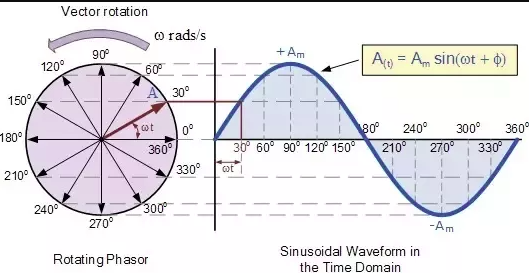
\includegraphics{physics/img/sinewave.png}
\item
  Waves are ultimately generated by oscillators.
\end{itemize}

\hypertarget{oscillators}{%
\section{Oscillators}\label{oscillators}}

\begin{figure}
\centering
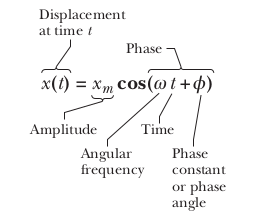
\includegraphics{img/oscillators.png}
\caption{oscillators}
\end{figure}

\begin{itemize}
\tightlist
\item
  It's similar to how we define a point in space in general except we're
  confined to an axis.
\item
  As a point moves through space we have acceleration and velocity that
  pop out of position at a given time
\item
  Oscillation is a repeated movement so we must return to an initial
  value, this is why the sine and cos functions are useful as they are
  defined on a circle.
\item
  The amplitude can be thought of as the radius of the circle
\end{itemize}

\hypertarget{notes}{%
\section{Notes}\label{notes}}

\begin{itemize}
\tightlist
\item
  22/09/22 13:46:02 Introduction to Electromagnetism

  \begin{itemize}
  \tightlist
  \item
    Apparently Ireland gets 10\% of the sun radiance in the winter
    months as it does in the summer months
  \item
    Force on a curved path. For each chunk of the path \(dl\) the net
    force may help you, or not. This is where we can use the dot product
    to figure out it's affect on \(dl\). It's a path integral, we don't
    have to consider it an arc because it's such a tiny chunk?
  \item
    Energy operates as a state function here too. Even though Work is
    derived from a path integral?
  \item
    Bigger the distance you do work over, the smaller the avg. work
    e.g.~catching a ball
  \item
    Time and symmetrical laws `causing' conservation. Emmy Noether.
  \item
    Try and review worked examples, to make sure they make sense.
  \end{itemize}
\item
  \href{https://www.youtube.com/watch?v=KGJqykotjog}{Thought this was a
  cool video}

  \begin{itemize}
  \tightlist
  \item
    Give's a good visualisation of de-localized electrons.
  \end{itemize}
\item
  Fields do the work. In the case of a circuit, the load is considered
  some resistance that energy is put into. It's the fields that the
  current generate that cause the electrons near the load to accelerate
  towards the ions of the load and do work. The electrons drift as well,
  but it's the field effect that travels at the speed of light?
\end{itemize}

\end{document}
